\documentclass[techdoc/techdoc.tex]{subfiles}

\begin{document}

\section{Vidareutveckling} \label{sec:5_develop}
För att underlätta vid vidareutveckling av applikationen har gruppen valt att
ta upp viss funktionalitet som de anser vara sannolika. Förhoppningen är att det
kan hjälpa utvecklare som är nya till systemet snabbt bli bekväma med systemet
och hur det kan breddas.

\subsection{Utökning av kategorier}
För att lägga till ytterligare kategorier i systemet så måste saker göras dels
hos journalen men även i alla de olika modulerna.

\begin{wrapfigure}{r}{0.3\linewidth}
    \vspace*{-5mm}
    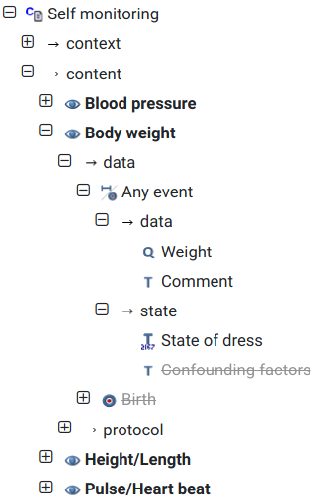
\includegraphics[width=\linewidth]{self_monitoring_archetype.png}
    \vspace*{-5mm}
    \caption{Nuvarande template för inrapportering.}
    \label{fig:sm-arch}
    \vspace*{-17mm}
\end{wrapfigure}

\subsubsection{Hos journalsystemet}
För att kunna lägga till en kategori måste det först finnas en lämplig
\texttt{Observable}-arketyp i openEHR. Den måste även läggas till i den
\emph{template} som applikationen används i. I figur \ref{fig:sm-arch} går det
att se den övergripande strukturen av den nuvarande \emph{template} som används
för att skapa kompositioner.

För att lägga till en ny kategori läggs en \emph{Observable} till under
\texttt{content}-grenen. Om arketypen innehåller klustret \emph{Medical Device}
bör den behållas så att applikationen kan ange insamlingsenhet.

När kategorin är tillagd i ens \emph{template} går den att ladda upp med en
POST-förfrågan till API-anropet \texttt{/template}.
\footnote{https://www.ehrscape.com/reference.html\#\_template}

\subsubsection{Ehr}
Nästa steg är att skapa en kategorispecifikation för kategorin. Dessa
definieras i filen \texttt{ehr-config.ts}. Som nämnt i avsnitt
\ref{sec:sys-datatype} måste denna innehålla ett id för kategorin, ett namn, en
beskrivning och en lista av datatypinstanser som beskriver varje element. Alla
id:n måste matcha de som används i JSON-formatet vid inrapportering. De
använder alltid samma namn som i \emph{template}:n, med skillnaden att alla
bokstäver är gemener samt att mellanrum ersätts med understreck.

Namnet och beskrivningen motsvaras av de svenska översättningarna i arketypen.
Id:t ska vara namnet av arketypen för kategorin fast med understreck,
exempelvis ersätts ``Body weight'' med \texttt{body\_weight}. Id:t bör även
läggas till i \texttt{Enum}:en \texttt{Categories} så att plattformarna kan
referera till den.

Slutligen måste en datatypinstans läggas till för varje element som
\emph{template}:n tillåter och som önskas användas. All information som ska gå
att hämta från en plattform eller kompletteras av användaren måste läggas till
som ett element i kategorispecifikationen.

I viktexemplet i figur \ref{fig:sm-arch} finns det tre element \texttt{weight},
\texttt{comment} och \texttt{state\_of\_dress}. Det måste utöver detta alltid
finnas ett fält för tid. Detta fält bör även ligga först så att sortering i
första hand utgår från mätvärdets tidpunkt.  Instanser för tid och kommentar
finns redan definierade i \texttt{ehr-config} som \texttt{TimeField} och
\texttt{CommentField}. Det finns även definerade instanser för att ange
information om mätenheten. Om kategorins arketyp innehåller klustret
\emph{Medical Device} bör dessa läggas till i kategorispecifikationen.

För resterande element; kontrollera att de datatyper som används är
implementerade i \texttt{datatype.ts}, lägg annars till datatyperna enligt
\ref{sec:dev-datatype}. Skapa därefter en instans av datatypen och lägg till
den i specifikationen. En \texttt{Enum} med datatypernas id bör även läggas
till för att undvika att stavfel sker när de ska refereras till av plattformens
implementation.

\subsubsection{Platform}
När kategorin finns i en \emph{template} hos journalsystemet och en motsvarande
kategorispecifikation har skapats återstår att implementera hämtning av
hälsodatan i aktuella plattformar. Detta är förstås väldigt beroende av
plattformens specifika implementation.

%Kanske ha en översiktlig beskrivning i teori-delen och länka till källor där?
\paragraph{Google Fit}
Mycket av det som tas upp nedan beskrivs i större detalj på
\url{https://developers.google.com/fit/rest/v1/reference/}.
Detta steget kan vara lite bökigt då inget annat sätt än att manuellt
identifiera dataströmmar för olika kategorier och de fält som innehåller
mätvärden hittats.  För att lägga till en kategori måste nedanstående göras i
\texttt{GfitService}:
\begin{itemize}
    \item Mappa Googles kategorinamn mot det interna kategorinamnet i
        \texttt{categoryDataTypeNames}. Googles standardtyper kan exempelvis
        hittas på
  \url{https://developers.google.com/fit/android/data-types#public_data_types}
    \item I konstruktorn initieras som tidigare nämnt
        \texttt{implementedCategories}. Här måste ny entry med den nya
        kategorin föras in. Förutom det interna kategorinamnet behövs en url
        till den dataström som data ska hämtas ifrån, samt en \texttt{Map} som
        beskriver vart de olika datatyperna för kategorin kan utläsas i det
        JSON-format som Google Fit returnerar.
\end{itemize}

Att lägga till url:en till den dataström som datan ska hämtas ifrån har i
projektet gjorts genom att gå in på
\url{https://developers.google.com/oauthplayground/}, välja 'Fitness v1' och de
scopes som är av intresse, och sedan skicka en \texttt{GET}-request för
metadata. Metadatan kan sedan genomsökas med exempelvis det kategorinamn som
ska implementeras. Det brukar finnas ett antal olika dataströmmar för varje
kategori, och i vår implementation används de dataströmmar som innehåller den
data som visas upp i Google Fit-appen. Dessa brukar ungefär vara på formen: \\
\texttt{derived:<kategorinamn>:com.google.android.gms:merge\_<kategorinamn>}.
Det bör även påpekas att endast de kategorier och dataströmmar som den
inloggade användaren aktivt laddat upp data på kommer att synas. Detta innebär
att det kan bli svårt att hitta vissa dataströmmar med denna metod. Under
projektet har tyvärr ingen dokumentation som visar alla existerande
dataströmmar hittats.

När den efterfrågade dataströmmen är funnen så är det sista steget att
identifiera vilka fält som innehåller data av intresse. För att hitta dessa
fält kan man hämta och granska den specifika dataströmmen för kategorin som ska
implementeras. Detta är exakt vad som görs i metoden \texttt{getData} när
kategorin sedan är färdigimplementerad. I OAuth playground görs det genom
följande anrop: \\
\texttt{https://www.googleapis.com/fitness/v1/users/me/dataSources/<dataström>/\\
datasets/startTimeNanos-endTimeNanos/?access\_token=<token>} \\ där
\texttt{startTimeNanos} och \texttt{endTimeNanos} är Unix-timestamp i
nanosekunder och \texttt{<token>} är den unika access token som gäller för
sessionen. Väl här så bör det synas vilket fält som innehåller själva
mätvärdet. Oftast är det under \texttt{point.value[0].fpval} eller liknande.
Några av de vanligaste fälten såsom tidpunkt och enhet är gemensamma för
samtliga kategorier och finns redan definierade i\\ \texttt{commonDataTypes}.
Mer noggrann dokumentation om olika fält och datasets finns på\\
\url{https://developers.google.com/fit/rest/v1/reference/users/dataSources/datasets}

Övrig dokumentation om \texttt{DataPoint}, \texttt{Dataset} och
\texttt{DataSource} som kan vara av intresse: \\
\url{https://developers.google.com/android/reference/com/google/android/gms/fitness/data/DataSource}
%https://www.googleapis.com/fitness/v1/users/me/dataSources/derived:com.google.weight:com.google.android.gms:merge_weight/datasets/0-1558185703/?access_token=<token>

%\subsubsection{GUI}
% TODO beskriva hur man lägger till ikon och mappar till kategorin

\subsection{Utökning av plattformar}
För att lägga till en ny plattform måste ändringar göras i flera av programmets
moduler.

\subsubsection{Platform}
För att implementera en ny plattform måste en ny service skapas i mappen
\texttt{platform} som ärver superklassen \texttt{Platform}. Därefter måste
metoderna \texttt{signIn}, \texttt{signOut} och \texttt{getData} och
\texttt{getAvailable} implementeras.

Metoden \texttt{signIn} ska autentisera användaren så att klienten därefter kan
anropa \texttt{getAvailable\-Categories} och \texttt{getData}.
\texttt{getAvailableCategories} ska returnera en \texttt{Observable} i form av
en lista av id:n för alla de kategorier som finns tillgängliga för användaren.
\texttt{getData} ska returnera en \texttt{Observable} i form av en lista av
\texttt{DataPoint}-instanser för alla datapunkter inom ett visst tidsintervall
för en kategori. Plattformen kommer antagligen inte föra in data i alla
tillgängliga fält, utan endast de som det finns data för. För exempelvis
kroppsvikt bör tid och vikt alltid fyllas i av plattformen. Kommentar och
klädsel kanske inte finns implementerat i plattformen, och kompletteras av
användaren om den önskar. Plattformen bör även fylla i fälten angående
mätenheten om den informationen finns tillgänglig.

Plattformen kan använda sig av fältet \texttt{implementedCategories} för att
mappa de implementerade kategoriernas id:n till funktioner som konverterar
kategorispecifik data från hälsoplattformens format till det interna formatet.
De id:n som används måste matcha kategorispecifikationernas id:n. Därmed bör
\texttt{Enum}:s med id:n från \texttt{ehr-config} användas för att se till att
det är exakt samma id.

\subsubsection{Conveyor}
När plattformen väl är implementerad återstår att se till att Conveyor har
tillgång till den. Detta görs genom att injicera Conveyor med den nya
plattformens service. För att åstadkomma detta måste klassen importeras och en
referens till klassen måste skapas i konstruktorn för Conveyor. Därefter måste
instansen av klassen läggas till i fältet \texttt{platforms} så att Conveyor
känner till att den finns. Ett id behöver även bestämmas för att kunna
specificera plattformen.

%\subsubsection{GUI}
% TODO beskriva hur man lägger till ikoner och mappar till plattformen

\subsection{Utökning av datatyper} \label{sec:dev-datatype}
Datatyper behöver dels definieras i Ehr-modulen men stöd behöver även skapas
i gränssnittet.

\subsubsection{Ehr}
Att skapa stöd för en ny datatyp innebär att skapa en ny klass. Klassen
definieras i \texttt{ehr/datatype.ts} och måste ärva den abstrakta superklassen
\texttt{DataType}. Nedan beskrivs hur varje metod därefter bör implementeras.

\paragraph{Konstruktorn} ska ta emot alla egenskaper som är specifika till en
datatyp. Exempelvis intervall och enhet för \texttt{DV\_QUANTITY}. Konstruktorn
sätter därefter dessa egenskaper i instansvariabler så att resterande metoder
kan använda dessa.

\paragraph{isValid} måste implementeras och har som uppgift att testa om ett
värde är giltigt eller inte. Värdet måste vara av rätt enhet och uppfylla alla
krav som satts av arketypen och kompositions-\emph{template}.

\paragraph{equal} ska jämföra två giltiga värden och avgöra om de är lika eller
inte. Om det räcker att jämföra värdena med \texttt{===} behöver den inte
implementeras eftersom den ärvs från \texttt{DataType}.

\paragraph{compare} ska jämföra två giltiga värden och avgöra vilket av värdena
som är störst. Om det första värdet är störst ska den returnera ett positivt
tal. Om det andra värdet är störst ska den returnera ett negativt tal och om
båda är exakt lika ska den returnera 0. Om det räcker att jämföra med
\texttt{<} och \texttt{>} behövs den ej implementeras eftersom den ärvs
från \texttt{DataType}.

\begin{wrapfigure}{r}{0.35\linewidth}
    \lstinputlisting[language=java]{techdoc/lst/json_weight.json}
    \caption{Exempel av en kompositon för kroppsvikt i JSON.}
    \label{fig:json_weight}
\end{wrapfigure}

\paragraph{Matematikfunktioner} behöver också implementeras om inte
implementationen från \texttt{DataType} är lämplig. Metoderna motsvarar
matematikfunktionerna i openEHR och inkluderar just nu \texttt{median},
\texttt{mean}, \texttt{total}, \texttt{min} och \texttt{max}. Metoderna ska ta
en lista av värden och returnera \emph{ett} värde som är en sammanställning av
alla värden med en viss funktion. Implementationen för \texttt{DataType} är
densamma för alla dessa; om alla värden är samma används det värdet, annars
används ett nollställt värde. Denna implementationen är lämplig för datatyper
som matematiska funktioner inte är rimliga för; exempelvis \texttt{DV\_TEXT}.
Om matematiska funktioner går att applicera på datatypen bör metoderna
implementeras så att beteendet från \texttt{DataType} inte används.

\paragraph{toRest} är en metod som måste implementeras. Den ska ta emot ett
giltigt värde och skapa ett motsvarande JSON-objekt som ska användas i anropet
till REST-API:n. Detta är väldigt beroende på datatypen och därför demonstreras
endast ett exempel. I figur \ref{fig:json_weight} visas ett exempel på hur en
komposition med ett värde för kroppsvikt kan se ut på JSON-formatet som används
mot API:n THINK-EHR. Varje element har en lista av objekt, och \texttt{toRest}
har i uppgift att ta ett giltigt värde och returnera det JSON-objektet som ska
läggas i listan. Exempelvis returnerar \texttt{toRest} för
\texttt{DataTypeQuantity} i detta fallet
\texttt{\{`|magnitude': 79.85, `|unit': `kg'\}}
% XXX possible to use actual quoutes in above??
då värdet ``79.85'' ges.

\subsubsection{GUI}
All hantering av data för gränssnittet sker inom modulen DataViewerModule.

\paragraph{DataTableComponent} måste uppdateras för att avgöra hur datatypen ska visas
och matas in.

I funktionen \texttt{getFormattedTextFromPoint} måste en sträng skapas utifrån
en datatyps värde som därefter ska visas i tabellen. Exempelvis blir ett värde
för datatypen \texttt{DataTypeQuantity} värdet i sig plus dess enhet.

I funktionen \texttt{getInputType} måste hur datatypen ska matas in i tabellen
specificeras genom att ange en sträng som motsvarar inmatningstypen, exempelvis
\texttt{'text-input'} och \texttt{'text'}. \texttt{'text'} används om datatypen
ej ska gå att ändra i tabellen. Därefter skapas ett \texttt{mat-form}-objekt
för varje typ av inmatning i komponentens HTML-fil
\texttt{data-table.component.html}.

%\paragraph{DataChartComponent}

%\subsection{BankID}
% TODO vad behöver göras, vart ska det göras?

%\subsection{Automatisk instansiering av kategorier}
% TODO vad behöver göras för att kunna automatisera hela instansieringen?

%\subsection{Specificera intervall eller punkt i komposition}
% TODO vad behöver göras, vart ska det göras?

\end{document}
